\documentclass[a4paper]{article}
\usepackage[fontset=macnew]{ctex}
\usepackage[a4paper,margin=0pt]{geometry}
\usepackage{xcolor}
\usepackage{amssymb}
\usepackage{graphicx}
\usepackage{tikz}
\usepackage{pagecolor}
\usepackage{array}
\usepackage{booktabs}
\usepackage{colortbl}
\usetikzlibrary{shapes.geometric, positioning, calc}

\definecolor{bgdark}{HTML}{1a1a2e}
\definecolor{cardbg}{HTML}{16213e}
\definecolor{accentgreen}{HTML}{2ecc71}
\definecolor{accentred}{HTML}{e74c3c}
\definecolor{accentyellow}{HTML}{f1c40f}
\definecolor{accentblue}{HTML}{3498db}
\definecolor{accentgray}{HTML}{95a5a6}
\definecolor{lighttext}{HTML}{ecf0f1}
\definecolor{subtletext}{HTML}{bdc3c7}
\definecolor{divider}{HTML}{2c3e50}

\pagecolor{bgdark}
\pagestyle{empty}
\setlength{\parindent}{0pt}
\setlength{\parskip}{0pt}

\begin{document}

\begin{tikzpicture}[remember picture, overlay]

%% ===== ROW 1: Header =====
\node[anchor=north, inner sep=0pt] at ([yshift=-6mm]current page.north) {%
\begin{minipage}[t]{\paperwidth}
\begin{center}

%% Status light
\begin{tikzpicture}
\fill[accentgreen] (0,0) circle (4mm);
\fill[bgdark] (0,0) circle (2.6mm);
\fill[accentgreen] (0,0) circle (1.6mm);
\end{tikzpicture}

\vspace{2mm}

{\color{lighttext}\fontsize{62}{74}\selectfont\bfseries delta0 量化数据报告}

\vspace{1mm}

{\color{subtletext}\fontsize{20}{26}\selectfont 2024-07-19 \,$\sim$\, 2026-07-21 \quad|\quad VQM 三因子多空策略}

\vspace{4mm}

{\color{accentgreen}\fontsize{24}{32}\selectfont\bfseries $\bigtriangleup$\, 增长 — 总收益 210.8\%，超额 186.7\%，回撤可控 $-$14.7\%}

\vspace{6mm}

%% Three big numbers
\setlength{\tabcolsep}{12pt}
\renewcommand{\arraystretch}{1}
\begin{tabular}{ccc}
{\color{accentgreen}\fontsize{52}{64}\selectfont\bfseries +210.8\%} &
{\color{accentred}\fontsize{52}{64}\selectfont\bfseries $-$14.7\%} &
{\color{accentblue}\fontsize{52}{64}\selectfont\bfseries 3.24} \\[3mm]
{\color{subtletext}\fontsize{15}{19}\selectfont 总收益} &
{\color{subtletext}\fontsize{15}{19}\selectfont 最大回撤} &
{\color{subtletext}\fontsize{15}{19}\selectfont 夏普比率} \\
\end{tabular}

\end{center}
\end{minipage}
};

%% Divider line below header
\draw[divider, line width=1.2pt]
  ([yshift=-66mm]current page.north west) --
  ([yshift=-66mm]current page.north east);

%% ===== ROW 2: Left | Center | Right =====

%% --- Left: Research Overview ---
\node[anchor=north west, inner sep=0pt] at ([xshift=6mm,yshift=-70mm]current page.north west) {%
\begin{minipage}[t]{50mm}
\begin{center}
{\color{accentblue}\fontsize{16}{20}\selectfont\bfseries 研究概述}
\end{center}
\vspace{3mm}
\color{subtletext}\fontsize{9.5}{13}\selectfont
\begin{tabular}{@{}p{11mm}p{36mm}@{}}
\textcolor{accentgreen}{\textbf{名称}} & delta0 VQM 策略 \\
\textcolor{accentgreen}{\textbf{目标}} & 跑赢沪深300，回撤 $\leq$ 15\% \\
\textcolor{accentgreen}{\textbf{逻辑}} & 动量+质量+价值三因子Z-score打分，月度调仓，15\%回撤控制 \\
\textcolor{accentgreen}{\textbf{市场}} & A股·日线 \\
\textcolor{accentgreen}{\textbf{周期}} & 2024-07-19\,$\sim$\,2026-07-21 \\
\textcolor{accentgreen}{\textbf{样本}} & 分析10只；底座20只 \\
\textcolor{accentgreen}{\textbf{基准}} & 沪深300指数 \\
\end{tabular}

\vspace{3mm}
{\color{subtletext}\fontsize{7.5}{10}\selectfont CSV:\,\texttt{price\_qfq.csv}\\\texttt{monthly\_selection.csv}}
\end{minipage}
};

%% --- Center: NAV vs Benchmark + Drawdown ---
\node[anchor=north, inner sep=0pt] at ([yshift=-70mm]current page.north) {%
\begin{minipage}[t]{92mm}
\begin{center}
{\color{accentblue}\fontsize{15}{19}\selectfont\bfseries 业绩与风险主图}
\end{center}
\vspace{1mm}
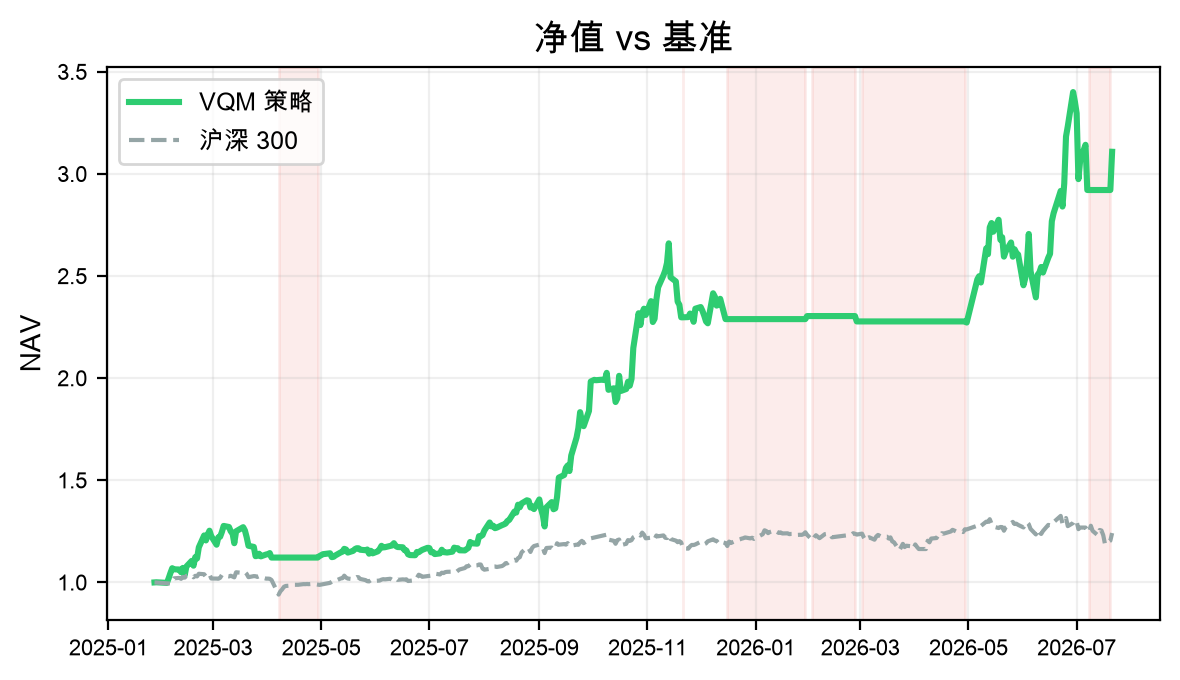
\includegraphics[width=92mm]{poster/fig_nav_benchmark.png}

\vspace{0.5mm}
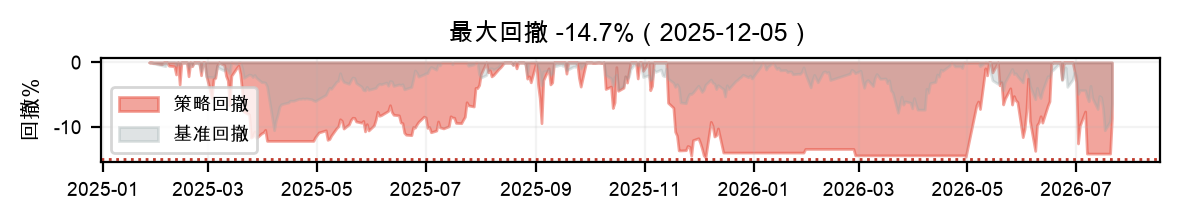
\includegraphics[width=92mm]{poster/fig_drawdown_strip.png}

\vspace{1mm}
{\color{subtletext}\fontsize{8.5}{11}\selectfont 超额收益主要出现在 \textcolor{accentgreen}{\textbf{2025 Q3 存储芯片主升浪}} 阶段}
\end{minipage}
};

%% --- Right: KPI Dashboard ---
\node[anchor=north east, inner sep=0pt] at ([xshift=-6mm,yshift=-70mm]current page.north east) {%
\begin{minipage}[t]{50mm}
\begin{center}
{\color{accentblue}\fontsize{16}{20}\selectfont\bfseries KPI 看板}
\end{center}
\vspace{2mm}

\setlength{\tabcolsep}{3pt}
\renewcommand{\arraystretch}{1.5}
\color{lighttext}\fontsize{9}{12}\selectfont
\begin{tabular}{@{}p{6mm}p{22mm}r@{}}
\toprule
\rowcolor{cardbg}
\multicolumn{3}{l}{\textcolor{accentgreen}{\textbf{\,收益}}} \\
\textcolor{accentgreen}{\textbf{收益}} & 总收益率 & \textcolor{accentgreen}{\textbf{+210.8\%}} \\
\textcolor{accentgreen}{\textbf{收益}} & 年化收益率 & \textcolor{accentgreen}{\textbf{+118.8\%}} \\
\rowcolor{cardbg}
\multicolumn{3}{l}{\textcolor{accentred}{\textbf{\,风险}}} \\
\textcolor{accentred}{\textbf{风险}} & 最大回撤 & \textcolor{accentred}{\textbf{$-$14.7\%}} \\
\textcolor{accentred}{\textbf{风险}} & 夏普比率 & \textcolor{accentblue}{\textbf{3.24}} \\
\textcolor{accentred}{\textbf{风险}} & 卡玛比率 & \textcolor{accentblue}{\textbf{8.07}} \\
\textcolor{accentred}{\textbf{风险}} & 年化波动 & \textcolor{accentred}{\textbf{36.0\%}} \\
\bottomrule
\end{tabular}

\vspace{2.5mm}
{\color{subtletext}\fontsize{7.5}{10}\selectfont 基准(沪深300):\\总收益+24.2\%\,夏普0.86\,波动17.0\%}
\end{minipage}
};

%% Divider line below row 2
\draw[divider, line width=1pt]
  ([yshift=-148mm]current page.north west) --
  ([yshift=-148mm]current page.north east);

%% ===== ROW 3: Left (heatmap) | Center (contribution) | Right (market env) =====

%% --- Left: Heatmap ---
\node[anchor=north west, inner sep=0pt] at ([xshift=6mm,yshift=-152mm]current page.north west) {%
\begin{minipage}[t]{50mm}
\begin{center}
{\color{accentblue}\fontsize{13}{17}\selectfont\bfseries 月度收益热力图}
\end{center}
\vspace{1mm}
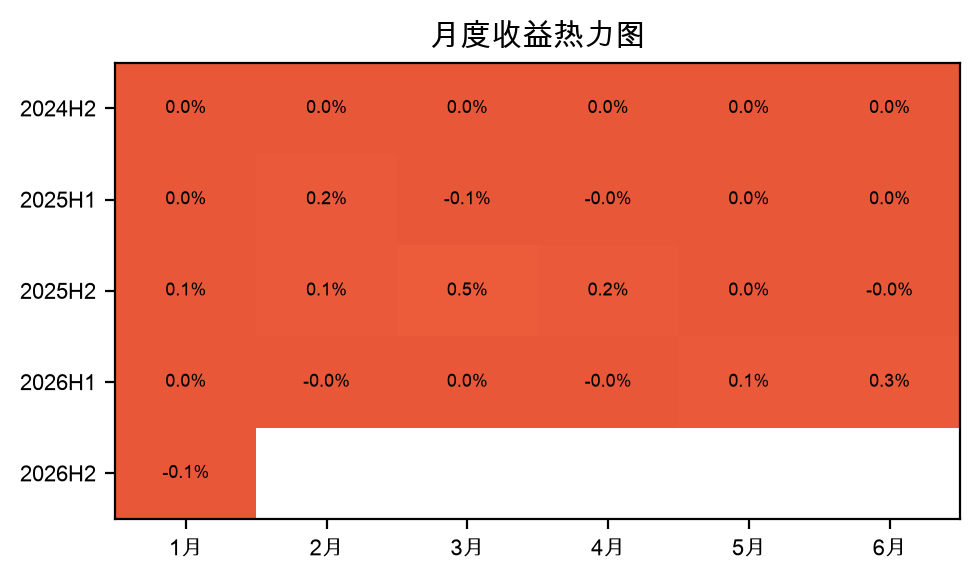
\includegraphics[width=50mm]{poster/fig_heatmap.png}
\end{minipage}
};

%% --- Center: Contribution bar ---
\node[anchor=north, inner sep=0pt] at ([yshift=-152mm]current page.north) {%
\begin{minipage}[t]{88mm}
\begin{center}
{\color{accentblue}\fontsize{13}{17}\selectfont\bfseries 个股贡献度}
\end{center}
\vspace{1mm}
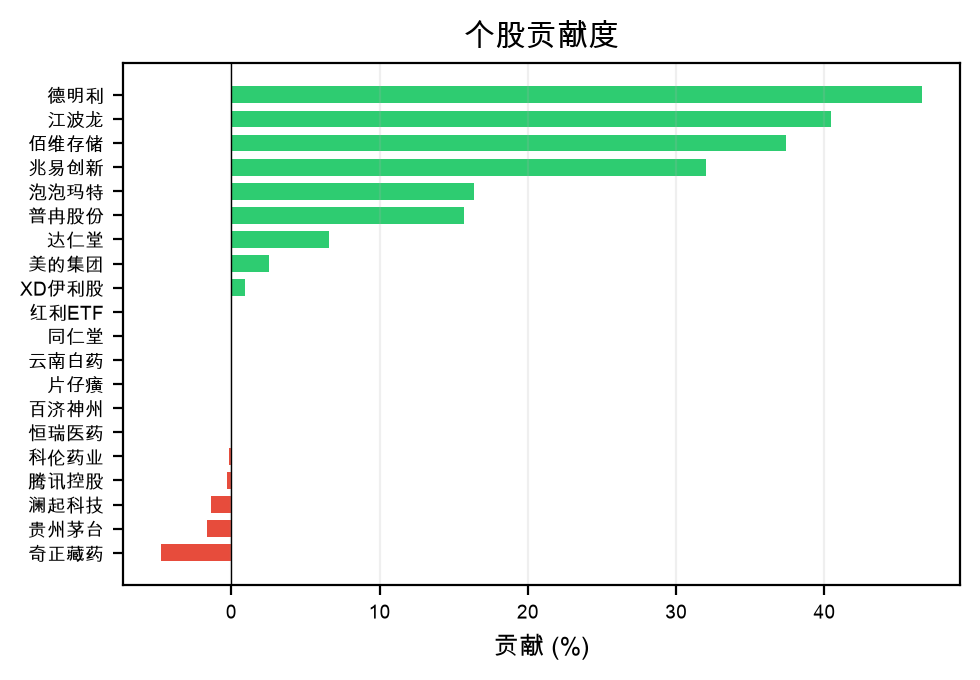
\includegraphics[width=82mm]{poster/fig_contrib.png}
\end{minipage}
};

%% --- Right: Market Environment Table ---
\node[anchor=north east, inner sep=0pt] at ([xshift=-6mm,yshift=-152mm]current page.north east) {%
\begin{minipage}[t]{50mm}
\begin{center}
{\color{accentblue}\fontsize{13}{17}\selectfont\bfseries 市场环境}
\end{center}
\vspace{1mm}

\setlength{\tabcolsep}{2pt}
\renewcommand{\arraystretch}{1.25}
\color{lighttext}\fontsize{7.5}{10}\selectfont
\begin{tabular}{@{}c c r r@{}}
\toprule
\textbf{季度} & \textbf{状态} & \textbf{策略} & \textbf{沪深300} \\
\midrule
25Q1 & 震荡 & \textcolor{accentgreen}{+13.7\%} & +1.8\% \\
25Q2 & 震荡 & \textcolor{accentgreen}{+2.7\%} & +1.2\% \\
25Q3 & 上涨 & \textcolor{accentgreen}{+69.8\%} & +17.7\% \\
25Q4 & 震荡 & \textcolor{accentgreen}{+14.9\%} & \textcolor{accentred}{$-$1.7\%} \\
26Q1 & 下跌 & \textcolor{accentgreen}{$-$0.5\%} & \textcolor{accentred}{$-$5.7\%} \\
26Q2 & 上涨 & \textcolor{accentgreen}{+47.3\%} & +10.0\% \\
26Q3 & 震荡 & \textcolor{accentred}{$-$5.7\%} & \textcolor{accentred}{$-$4.4\%} \\
\bottomrule
\end{tabular}
\end{minipage}
};

%% ===== ROW 4: Conclusions & Action (bottom) =====

\draw[divider, line width=1pt]
  ([yshift=44mm]current page.south west) --
  ([yshift=44mm]current page.south east);

\node[anchor=south west, inner sep=0pt] at ([xshift=6mm,yshift=6mm]current page.south west) {%
\begin{minipage}[t]{0.30\paperwidth}
{\color{accentgreen}\fontsize{11}{15}\selectfont\bfseries \checkmark\, 优势}
\vspace{1.5mm}

{\color{lighttext}\fontsize{8.5}{11.5}\selectfont
1.\,三因子Z-score打分有效捕捉存储芯片主升浪\\[1mm]
2.\,15\%回撤控制将$-$48\%回撤截断至$-$14.7\%
}
\end{minipage}
};

\node[anchor=south, inner sep=0pt] at ([yshift=6mm]current page.south) {%
\begin{minipage}[t]{0.26\paperwidth}
{\color{accentred}\fontsize{11}{15}\selectfont\bfseries $\times$\, 不足}
\vspace{1.5mm}

{\color{lighttext}\fontsize{8.5}{11.5}\selectfont
1.\,收益高度集中于半导体板块（Top3占124\%）\\[1mm]
2.\,32\%空仓时间错过部分反弹机会
}
\end{minipage}
};

\node[anchor=south east, inner sep=0pt] at ([xshift=-6mm,yshift=6mm]current page.south east) {%
\begin{minipage}[t]{0.30\paperwidth}
{\color{accentyellow}\fontsize{11}{15}\selectfont\bfseries $\rightarrow$\, 下一步}
\vspace{1.5mm}

{\color{lighttext}\fontsize{8.5}{11.5}\selectfont
\textcolor{accentgreen}{\textbf{[立即]}}\,加入风格约束限制进攻型持仓\\[1mm]
\textcolor{accentyellow}{\textbf{[本周]}}\,测试延迟切换ETF方案\\[1mm]
\textcolor{accentblue}{\textbf{[持续]}}\,滚动更新PE/ROE因子
}
\end{minipage}
};

%% Bottom-most: disclaimer + logo
\node[anchor=south west, inner sep=0pt] at ([xshift=6mm,yshift=1mm]current page.south west) {%
\begin{minipage}[t]{0.60\paperwidth}
{\color{subtletext}\fontsize{5.5}{7.5}\selectfont
本量化数据报告不构成投资建议，仅个人间讨论，切勿模仿！本报告已获得版权保护，属于创作者和程翊博所有，切勿盗用商用，违者必究，需负相应的法律责任。}
\end{minipage}
};

\node[anchor=south east, inner sep=0pt] at ([xshift=-6mm,yshift=0mm]current page.south east) {%
\begin{minipage}[t]{0.20\paperwidth}
\raggedleft

\includegraphics[width=20mm]{logo.png}\\[0.5mm]
{\color{subtletext}\fontsize{5.5}{7.5}\selectfont 数据来源：AKShare\,/\,Tushare}
\end{minipage}
};

\end{tikzpicture}

\end{document}
